\documentclass[12pt, paper=a4]{article}
\usepackage[utf8]{inputenc}
\usepackage[german]{babel}
\usepackage{mathrsfs}
\usepackage{amsmath}
\usepackage{amssymb}
\usepackage{listings}
\usepackage{graphicx}
\usepackage{fancyhdr}

\setlength{\parindent}{0pt}

\author{Mareike G\"ottsch, 6695217, Gruppe 2\\Paul H\"olzen, 6673477, Gruppe 1\\Sven Schmidt, 6217064, Gruppe 1}

\title{FGI 2 Hausaufgaben 6}

\rhead{M. G\"ottsch, G-2; P. H\"olzen, G-1; S. Schmidt, G-1}
\pagestyle{fancy}
\begin{document}
\maketitle

\section*{Aufgabe 7.3}
\subsection*{1.}
\begin{figure}[h!]
\centering
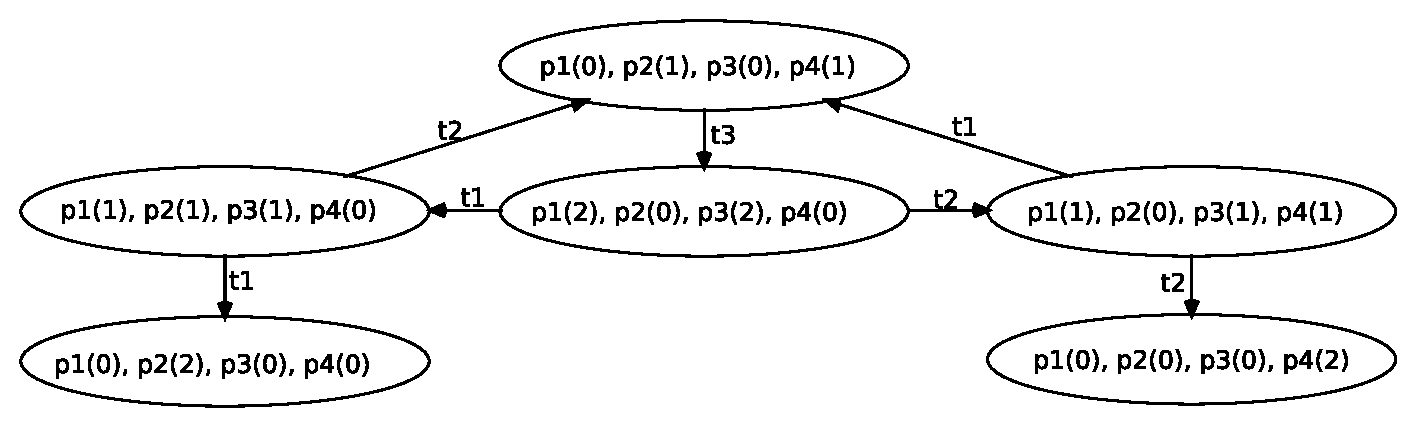
\includegraphics[scale=0.6]{Erreichbarkeitsgraph7-3-1.pdf}
\caption{Erreichbarkeitsgraph}
\end{figure}

\subsection*{2.}
$\sigma = t_3t_1t_2t_3t_1t_2t_3$\\

\subsection*{3.}
Das Netz ist nicht verklemmungsfrei, da für die Markierung $m_1 = p1(0)p2(2)p3(0)p4(0)$ bzw. $m_2 = p1(0)p2(0)p3(0)p4(2)$ keine Transition mehr schalten kann. Aus diesem Grund ist das Netz auch nicht lebendig. Auch die Reversibilität ist nicht gegeben, da in den verklemmten Markierungen auch kein Pfad existiert, der die Anfangsmarkierung wiederherstellen könnte.\\

\subsection*{4.}

\subsection*{5.}

\section*{Aufgabe 7.5}

\end{document}